\documentclass[tikz]{standalone}
\usepackage{tikz}
\usetikzlibrary{calc}
\usepackage{xcolor}
% For formatting pseudocode
\usepackage{listings}

\definecolor{mGreen}{rgb}{0,0.6,0}
\definecolor{mGray}{rgb}{0.5,0.5,0.5}
\definecolor{mPurple}{rgb}{0.58,0,0.82}
\definecolor{backgroundColour}{rgb}{0,0,0}

\lstdefinestyle{CStyle}{
    %backgroundcolor=\color{backgroundColour},
    commentstyle=\color{mGreen},
    keywordstyle=\color{magenta},
    numberstyle=\tiny\color{mGray},
    stringstyle=\color{mPurple},
    basicstyle=\footnotesize,
    breakatwhitespace=false,
    breaklines=true,
    captionpos=b,
    keepspaces=true,
    numbers=left,
    numbersep=5pt,
    showspaces=false,
    showstringspaces=false,
    showtabs=false,
    tabsize=2,
    language=C
}

\newsavebox\mybox


% Define function box macro
\newcommand{\functionBox}[7]{%
  \begin{scope}[shift={(#1, #2)}]%
    \def\boxwidth{#3}
    \def\titleheight{#4}
    \def\bodyheight{#5}

    \draw[thick] (0, 0) rectangle (\boxwidth, -\titleheight - \bodyheight);
    \draw (0, -\titleheight) -- (\boxwidth, -\titleheight);

    \node[anchor=mid, align=center]
      at (\boxwidth/2, -\titleheight/2)
      {\textbf{#6}};

    \node[anchor=north west, align=left, font=\footnotesize]
      at (0.1, -\titleheight - 0.1) {
%        \begin{minipage}[t][#5][t]{\boxwidth-0.2cm}
%          #7
%        \end{minipage}

        #7
      };
  \end{scope}%
}

\begin{document}

\begin{lrbox}{\mybox}
\begin{lstlisting}[style=CStyle]
#include <stdio.h>
int main(void)
{
   printf("Hello World!");
}
\end{lstlisting}
\end{lrbox}



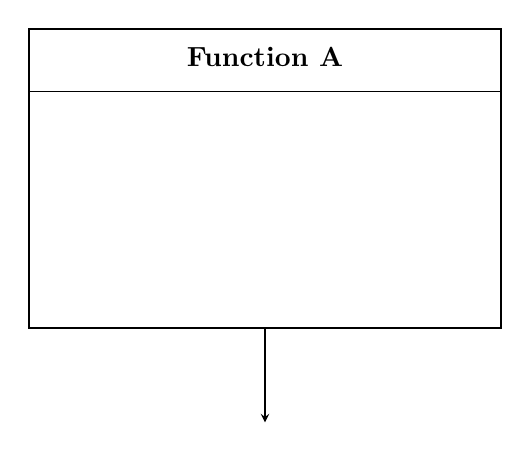
\begin{tikzpicture}[>=stealth]
  % Define C and Assembly pseudocode
%
%  \newcommand{\functionBPseudocode}{
%\begin{lstlisting}[language={[x86masm]Assembler}]
%_start:
%  mov eax, 42   ; Load immediate value
%  call funcB    ; Call another function
%\end{lstlisting}
%}
%
  % Create boxes with pseudocode
  \functionBox{0}{0}{6.0}{0.8}{3.0}{Function A}{\usebox\mybox}
  %\functionBox{0}{-5}{6.0}{0.8}{3.0}{Function B}{\functionAPseudocode}

  % Connect the boxes
  \draw[->] (3, -3.8) -- (3, -5);
\end{tikzpicture}


\end{document}

